%%%% This is based on the Beamer example was created by LianTze Lim, April 2017.

\documentclass[14pt]{beamer}

%%%%%%%%%%%%%%%%%%%%%%%%%%%%%%%%%%%%%%%%%%%%%%%%%%%%%%%%%%%%%%%%%%%%%%%%%%%%%%%%

    \usepackage[english]{babel}
    \usepackage[utf8]{inputenc}
    \usepackage[T1]{fontenc}
    \usepackage{lmodern}
    \usepackage{textcomp}
    \usepackage[cm]{sfmath}
    \usepackage[euler]{textgreek}

    \usepackage{xfrac}

    %% Set the left and right margins
    \setbeamersize{text margin left=1em,text margin right=1em}

    %% Fonts
    \setbeamerfont{title}{series=\bfseries,size=\huge}
    \setbeamerfont{subtitle}{series=\bfseries,size=\large}
    \setbeamerfont{date}{size=\footnotesize}
    \setbeamerfont{frametitle}{series=\bfseries,size=\large}
    \setbeamerfont{block title}{series=\bfseries,size=\large}
    \setbeamerfont{footline}{size=\normalsize}

    %% Colors
    \setbeamercolor{background canvas}{bg=white!5!black}    % Blackboard
    \setbeamercolor{structure}{fg=white!95!black}           % Chalk
    \usebeamercolor{structure}
    \setbeamercolor{normal text}{fg=structure.fg}

    %% Add a line after the frametitle
    \setbeamertemplate{frametitle}[default][left,leftskip=1ex]
    \addtobeamertemplate{frametitle}{}{\vspace*{-1ex}\rule{\textwidth}{2pt}}

    %% Use circular discs as itemized list markers
    \setbeamertemplate{itemize items}[circle]

    %% Remove default navigation symbols
    \setbeamertemplate{navigation symbols}{}

    %% Remove the footline
    \setbeamertemplate{footline}{}

    % MMACa Logo
    \setlength{\fboxsep}{3pt}
    \setlength{\fboxrule}{0.75pt}


%%%%%%%%%%%%%%%%%%%%%%%%%%%%%%%%%%%%%%%%%%%%%%%%%%%%%%%%%%%%%%%%%%%%%%%%%%%%%%%%

\title{The Egyptian Tangram\vspace{-0.25em}}
\author{
    
\includegraphics[height=18ex]{figures/figure001a.pdf}\\
    \;\;{\small \textcopyright\ \href{https://github.com/CarlosLunaMota}{Carlos Luna-Mota}}\\
    \vspace{0.55em}
    \href{https://mmaca.cat/}{\large \framebox{\textbf{mmaca}}}\\
    \vspace{-1.85em}}
\date{\today}


\begin{document}

    %%%%%%%%%%%%%%%%%%%%%%%%%%%%%%%%%%%%%%%%%%%%%%%%%%%%%%%%%%%%%%%%%%%%%%%%%%%%

    \begin{frame}
      \titlepage
    \end{frame}

    %%%%%%%%%%%%%%%%%%%%%%%%%%%%%%%%%%%%%%%%%%%%%%%%%%%%%%%%%%%%%%%%%%%%%%%%%%%%

    \begin{frame}{}
        \begin{center}
            \textbf{\huge The Egyptian Tangram}
        \end{center}
    \end{frame}

    %%%%%%%%%%%%%%%%%%%%%%%%%%%%%%%%%%%%%%%%%%%%%%%%%%%%%%%%%%%%%%%%%%%%%%%%%%%%

    \begin{frame}{The Egyptian Tangram}
        \begin{center}
            
\includegraphics[height=20ex]{figures/figure001a.pdf} \\

            \bigskip

            A square dissection firstly proposed as a tangram in:

            \bigskip

            {\footnotesize Luna-Mota, C. (2019) \emph{``El tangram egipci: diari de disseny''} Nou Biaix, 44}
        \end{center}
    \end{frame}

    %%%%%%%%%%%%%%%%%%%%%%%%%%%%%%%%%%%%%%%%%%%%%%%%%%%%%%%%%%%%%%%%%%%%%%%%%%%%

    \begin{frame}{Origins}
        \begin{center}
            The Egyptian Tangram inspiration comes from\\the study of two other 5-piece tangrams...

            \bigskip

            
\includegraphics[height=18ex]{figures/figure000a.pdf} \qquad 
\includegraphics[height=18ex]{figures/figure000b.pdf} \\

            \bigskip

            {\small The ``Five Triangles'' \& ``Greek-Cross'' tangrams}
        \end{center}
    \end{frame}

    %%%%%%%%%%%%%%%%%%%%%%%%%%%%%%%%%%%%%%%%%%%%%%%%%%%%%%%%%%%%%%%%%%%%%%%%%%%%

    \begin{frame}{Origins}
        \begin{center}
            ...and their underlying grids\\\phantom{the study of two other 5-piece tangrams...}

            \bigskip

            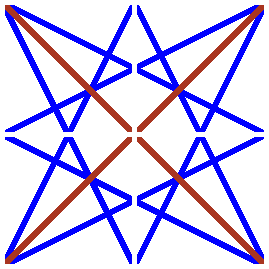
\includegraphics[height=18ex]{figures/figure000d.pdf} \qquad 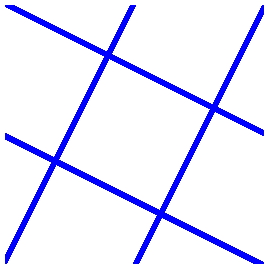
\includegraphics[height=18ex]{figures/figure000c.pdf} \\

            \bigskip

            {\small The ``Five Triangles'' \& ``Greek-Cross'' underlying grids}
        \end{center}
    \end{frame}

    %%%%%%%%%%%%%%%%%%%%%%%%%%%%%%%%%%%%%%%%%%%%%%%%%%%%%%%%%%%%%%%%%%%%%%%%%%%%

    \begin{frame}{Design Process}
        \begin{center}
            The Egyptian Tangram is the result of\\an heuristic incremental design process:

            \bigskip\bigskip\bigskip

            
\includegraphics[height=10ex]{figures/figure001e.pdf} \quad 
\includegraphics[height=10ex]{figures/figure001d.pdf} \quad 
\includegraphics[height=10ex]{figures/figure001c.pdf} \quad 
\includegraphics[height=10ex]{figures/figure001b.pdf} \\

            \bigskip\bigskip\bigskip

            {\small Take a square and keep adding ``the most interesting straight cut'' until you have a dissection with 5 or more pieces.}
        \end{center}
    \end{frame}

    %%%%%%%%%%%%%%%%%%%%%%%%%%%%%%%%%%%%%%%%%%%%%%%%%%%%%%%%%%%%%%%%%%%%%%%%%%%%

    \begin{frame}{Design Process}
        \begin{center}
            
\includegraphics[height=18ex]{figures/figure001b.pdf}
        \end{center}

        To make an Egyptian Tangram from a square:

        {\small \begin{enumerate}
            \item Connect the midpoint of the lower side with the upper corners.
            \item Connect the midpoint of the left side with the top right corner.
        \end{enumerate}}
    \end{frame}

    %%%%%%%%%%%%%%%%%%%%%%%%%%%%%%%%%%%%%%%%%%%%%%%%%%%%%%%%%%%%%%%%%%%%%%%%%%%%

    \begin{frame}{Antecedents}
        \begin{center}
            It turns out that this figure is not new...

            \bigskip\medskip

            {\footnotesize Detemple, D. \& Harold, S. (1996) \emph{``A Round-Up of Square Problems''}}\\

            \bigskip

            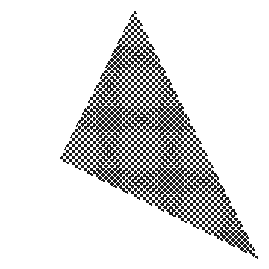
\includegraphics[height=14ex]{figures/figure000f.pdf}\\[-1ex]{\footnotesize \textbf{Problem 3}}

            \bigskip

            ...but, to the best of our knowledge,\\nobody used it before \textbf{as a tangram}
        \end{center}
    \end{frame}

    %%%%%%%%%%%%%%%%%%%%%%%%%%%%%%%%%%%%%%%%%%%%%%%%%%%%%%%%%%%%%%%%%%%%%%%%%%%%

    \begin{frame}{Antecedents}
        \begin{center}
            The name is not new either...

            \bigskip \bigskip

            
\includegraphics[height=15ex]{figures/figure000e.pdf}

            \medskip

            {\footnotesize This dissection is often called ``Egyptian Puzzle'' or ``Egyptian Tangram''}

            \bigskip \bigskip

            ...but there is a good reason to consider\\ our dissection the real ``Egyptian Tangram''\\{\footnotesize (even if it was designed in Barcelona)}
        \end{center}
    \end{frame}

    %%%%%%%%%%%%%%%%%%%%%%%%%%%%%%%%%%%%%%%%%%%%%%%%%%%%%%%%%%%%%%%%%%%%%%%%%%%%

    \begin{frame}{Antecedents}
        \begin{center}
            The underlying grid is also a well known figure:

            \bigskip\bigskip\bigskip

            
\includegraphics[height=15ex]{figures/figure002b.pdf}\\

            \bigskip\bigskip

            {\footnotesize Brunés, T. (1967) \emph{``The Secrets of Ancient Geometry -- and Its Use''}}

            \medskip

            {\footnotesize Bankoff, L. \& W. Trigg, C. (1974) \emph{``The Ubiquitous 3:4:5 Triangle''}}
        \end{center}
    \end{frame}

    %%%%%%%%%%%%%%%%%%%%%%%%%%%%%%%%%%%%%%%%%%%%%%%%%%%%%%%%%%%%%%%%%%%%%%%%%%%%

    \begin{frame}{The pieces}
        \begin{center}

            \begin{minipage}{17.5ex}\vspace{2ex}
                
\includegraphics[height=17ex]{figures/figure001a.pdf}\\
            \end{minipage}\begin{minipage}{30ex}
                \footnotesize
                \begin{itemize}
                    \item Just five pieces
                    \item All pieces are different
                    \item All pieces are asymmetric
                    \item Areas are integer and not \emph{too different}
                    \item All sides are multiples of $1$ or $\sqrt{5}$
                    \item All angles are linear combinations of $90^\circ$ and \textalpha\ $= \arctan{\!\left(\tfrac{1}{2}\right)} \approx 26,565^\circ$
                \end{itemize}
            \end{minipage}

            \smallskip

            {\footnotesize
            \begin{tabular}{c|c|l|l}
                \;\;\textbf{Name}\;\; & \;\;\textbf{Area}\;\; & \;\;\textbf{Sides}          & \;\;\textbf{Angles} \\ \hline
                \textbf{T1}   & $1$           & \;\;$1,\; 2,\; \sqrt{5}$          & \;\;$90,\; \text{\textalpha},\; 90\!-\!\text{\textalpha}$   \\ \hline
                \textbf{T4}   & $4$           & \;\;$2,\; 4,\; 2\sqrt{5}$         & \;\;$90,\; \text{\textalpha},\; 90\!-\!\text{\textalpha}$   \\ \hline
                \textbf{T5}   & $5$           & \;\;$\sqrt{5},\; 2\sqrt{5},\; 5$  & \;\;$90,\; \text{\textalpha},\; 90\!-\!\text{\textalpha}$   \\ \hline
                \textbf{T6}   & $6$           & \;\;$3,\; 4,\; 5$                 & \;\;$90,\; 90\!-\!2\text{\textalpha},\; 2\text{\textalpha}$ \\ \hline
                \textbf{Q4}   & $4$           & \;\;$1,\; 3,\; \sqrt{5},\; \sqrt{5}$\;\; & \;\;$90,\; 90\!-\!\text{\textalpha},\; 90,\; 90\!+\!\text{\textalpha}$\;\;
            \end{tabular}}
        \end{center}
    \end{frame}

    %%%%%%%%%%%%%%%%%%%%%%%%%%%%%%%%%%%%%%%%%%%%%%%%%%%%%%%%%%%%%%%%%%%%%%%%%%%%

    \begin{frame}{The pieces}
        \begin{center}
            Although all pieces are asymmetric and different,\\they often combine to make symmetric shapes

            \bigskip \bigskip

            \includegraphics[height=7ex]{figures/figure010a.pdf}\quad\includegraphics[height=7ex]{figures/figure010b.pdf}\quad\includegraphics[height=7ex]{figures/figure010c.pdf}\qquad
            \includegraphics[height=7ex]{figures/figure010h.pdf}\quad\includegraphics[height=7ex]{figures/figure010i.pdf} \\ \bigskip
            \includegraphics[height=7ex]{figures/figure010d.pdf}\quad\includegraphics[height=7ex]{figures/figure010f.pdf} \quad \includegraphics[height=7ex]{figures/figure010e.pdf}\quad\includegraphics[height=7ex]{figures/figure010g.pdf} \\ \bigskip
            \includegraphics[height=3ex]{figures/figure010k.pdf}\quad\includegraphics[height=3ex]{figures/figure010j.pdf} \\ \medskip
            \includegraphics[height=3ex]{figures/figure010m.pdf}\quad\includegraphics[height=3ex]{figures/figure010l.pdf} \\
        \end{center}
    \end{frame}

    %%%%%%%%%%%%%%%%%%%%%%%%%%%%%%%%%%%%%%%%%%%%%%%%%%%%%%%%%%%%%%%%%%%%%%%%%%%%

    \begin{frame}{The pieces}
        \begin{center}
            This means that it is very rare for an Egyptian Tangram figure to have a unique solution

            \bigskip \bigskip

            \includegraphics[height=12ex]{figures/figure011a.pdf}\quad\includegraphics[height=12ex]{figures/figure011b.pdf}\quad\includegraphics[height=12ex]{figures/figure011c.pdf} \\

            \vspace{2em}

            {\footnotesize There are three different solutions for the square and, in all three cases,\\two of the corners of the square are built as a sum of acute angles!}
        \end{center}
    \end{frame}

    %%%%%%%%%%%%%%%%%%%%%%%%%%%%%%%%%%%%%%%%%%%%%%%%%%%%%%%%%%%%%%%%%%%%%%%%%%%%

    \begin{frame}{The pieces}
        \begin{center}
            The assymetry of the pieces also implies that each solution belongs to one of these equivalence classes:

            \bigskip\bigskip

            \begin{tabular}{llllrrrr}
                \includegraphics[scale=0.15]{figures/figure021nnnnn.pdf} &
                \includegraphics[scale=0.15]{figures/figure021rnnnn.pdf} &
                \includegraphics[scale=0.15]{figures/figure021nrnnn.pdf} &
                \includegraphics[scale=0.15]{figures/figure021rrnnn.pdf} \!\!\!&\!\!\!
                \includegraphics[scale=0.15]{figures/figure021nnrrr.pdf} &
                \includegraphics[scale=0.15]{figures/figure021rnrrr.pdf} &
                \includegraphics[scale=0.15]{figures/figure021nrrrr.pdf} &
                \includegraphics[scale=0.15]{figures/figure021rrrrr.pdf} \\[1.5ex]
                \includegraphics[scale=0.15]{figures/figure021nnnnr.pdf} &
                \includegraphics[scale=0.15]{figures/figure021rnnnr.pdf} &
                \includegraphics[scale=0.15]{figures/figure021nrnnr.pdf} &
                \includegraphics[scale=0.15]{figures/figure021rrnnr.pdf} \!\!\!&\!\!\!
                \includegraphics[scale=0.15]{figures/figure021nnrrn.pdf} &
                \includegraphics[scale=0.15]{figures/figure021rnrrn.pdf} &
                \includegraphics[scale=0.15]{figures/figure021nrrrn.pdf} &
                \includegraphics[scale=0.15]{figures/figure021rrrrn.pdf} \\[1.2ex]
                \includegraphics[scale=0.15]{figures/figure021nnnrn.pdf} &
                \includegraphics[scale=0.15]{figures/figure021rnnrn.pdf} &
                \includegraphics[scale=0.15]{figures/figure021nrnrn.pdf} &
                \includegraphics[scale=0.15]{figures/figure021rrnrn.pdf} \!\!\!&\!\!\!
                \includegraphics[scale=0.15]{figures/figure021nnrnr.pdf} &
                \includegraphics[scale=0.15]{figures/figure021rnrnr.pdf} &
                \includegraphics[scale=0.15]{figures/figure021nrrnr.pdf} &
                \includegraphics[scale=0.15]{figures/figure021rrrnr.pdf} \\[1.5ex]
                \includegraphics[scale=0.15]{figures/figure021nnnrr.pdf} &
                \includegraphics[scale=0.15]{figures/figure021rnnrr.pdf} &
                \includegraphics[scale=0.15]{figures/figure021nrnrr.pdf} &
                \includegraphics[scale=0.15]{figures/figure021rrnrr.pdf} \!\!\!&\!\!\!
                \includegraphics[scale=0.15]{figures/figure021nnrnn.pdf} &
                \includegraphics[scale=0.15]{figures/figure021rnrnn.pdf} &
                \includegraphics[scale=0.15]{figures/figure021nrrnn.pdf} &
                \includegraphics[scale=0.15]{figures/figure021rrrnn.pdf} \\
            \end{tabular}

            \bigskip

            {\footnotesize You cannot transform one of these figures into another without flipping a piece}
        \end{center}
    \end{frame}

    %%%%%%%%%%%%%%%%%%%%%%%%%%%%%%%%%%%%%%%%%%%%%%%%%%%%%%%%%%%%%%%%%%%%%%%%%%%%

        \begin{frame}{Why we called it the \emph{Egyptian} Tangram?}
        \begin{center}
            The smallest pieces of the Chinese and Greek-Cross tangrams can be used to build all the other pieces...

            \bigskip \bigskip

            \includegraphics[height=15ex]{figures/figure003c.pdf}\quad\includegraphics[height=15ex]{figures/figure003a.pdf}\quad\includegraphics[height=15ex]{figures/figure003b.pdf} \\

            \bigskip \bigskip

            ...but you cannot do the same with\\the Egyptian Tangram because of T6
        \end{center}
    \end{frame}

    %%%%%%%%%%%%%%%%%%%%%%%%%%%%%%%%%%%%%%%%%%%%%%%%%%%%%%%%%%%%%%%%%%%%%%%%%%%%

    \begin{frame}{Why we called it the \emph{Egyptian} Tangram?}
        \begin{center}
            {\small Initially, T6 was considered as the \emph{leftover} piece that results from cutting all these $1\!\!:\!\!2\!\!:\!\!\sqrt{5}$ triangles from the borders of the square.\\But it turned out to be a very well known triangle...}

            \bigskip \bigskip

            \includegraphics[height=15ex]{figures/figure003a.pdf} \\

            \bigskip \bigskip

            ...the \textbf{Egyptian} Triangle ($3\!\!:\!\!4\!\!:\!\!5$)\\{\small and, hence, the name}
        \end{center}
    \end{frame}

    %%%%%%%%%%%%%%%%%%%%%%%%%%%%%%%%%%%%%%%%%%%%%%%%%%%%%%%%%%%%%%%%%%%%%%%%%%%%

    \begin{frame}{}
        \begin{center}
            \textbf{\Huge Puzzles \& Activities}\\
        \end{center}
    \end{frame}

    %%%%%%%%%%%%%%%%%%%%%%%%%%%%%%%%%%%%%%%%%%%%%%%%%%%%%%%%%%%%%%%%%%%%%%%%%%%%

    \begin{frame}{Realistic figures}
        \vspace{-1em}
        \begin{center}
            \quad Use all five pieces to make these figures:

            \vspace{-0.3em}

            {\footnotesize
            \begin{tabular}{ccccc}
                \includegraphics[scale=0.20]{figures/figure016bp.pdf}\;\;\;\;\; &
                \includegraphics[scale=0.20]{figures/figure016c.pdf}  &
                \includegraphics[scale=0.20]{figures/figure016r.pdf}  &
                \includegraphics[scale=0.20]{figures/figure016ad.pdf} &
                \;\;\includegraphics[scale=0.20]{figures/figure016bc.pdf} \\
                Lightning & Sailing ship & Bow tie & Wooden hut & Caltrop \\[4ex]
                \includegraphics[scale=0.20]{figures/figure016b.pdf}  &
                \includegraphics[scale=0.20]{figures/figure016p.pdf}  &
                \includegraphics[scale=0.20]{figures/figure016a.pdf}  &
                \includegraphics[scale=0.20]{figures/figure016f.pdf}  &
                \includegraphics[scale=0.20]{figures/figure016ay.pdf} \\
                Snowmobile & Candle & \;Viking hat & Diamond & Moses basket\\[3.5ex]
                \includegraphics[scale=0.20]{figures/figure016g.pdf}  &
                \includegraphics[scale=0.20]{figures/figure016aw.pdf} &
                \!\includegraphics[scale=0.20]{figures/figure016bd.pdf} \!&
                \includegraphics[scale=0.20]{figures/figure012t.pdf} &
                \includegraphics[scale=0.20]{figures/figure016ae.pdf} \\
                Erlenmeyer & 3D brick\;\; & Witch hat & Arrow Sign & Sailboat\\
            \end{tabular}}
        \end{center}
    \end{frame}

    %%%%%%%%%%%%%%%%%%%%%%%%%%%%%%%%%%%%%%%%%%%%%%%%%%%%%%%%%%%%%%%%%%%%%%%%%%%%

    \begin{frame}{Realistic figures}
        \vspace{-1em}
        \begin{center}
            \quad Use all five pieces to make these figures:

            \vspace{-0.8em}

            {\footnotesize
            \begin{tabular}{ccccc}
                \includegraphics[scale=0.20]{figures/figure016aa.pdf}\; &
                \;\includegraphics[scale=0.20]{figures/figure016bf.pdf}\;  &
                \;\!\includegraphics[scale=0.20]{figures/figure016v.pdf}\! &
                \;\includegraphics[scale=0.20]{figures/figure016al.pdf}\;  &
                \;\includegraphics[scale=0.20]{figures/figure016h.pdf}\; \\
                Gnome & Handmaid & \!\!Mountain range\!\! & Fish tail & Teddy bear \\[1.5ex]
                \;\includegraphics[scale=0.20]{figures/figure016ao.pdf}\; &
                \;\;\;\includegraphics[scale=0.20]{figures/figure016x.pdf}\; &
                \;\!\!\!\!\includegraphics[scale=0.20]{figures/figure016ag.pdf}\; &
                \;\includegraphics[scale=0.20]{figures/figure016ac.pdf}\; &
                \;\includegraphics[scale=0.20]{figures/figure016ap.pdf}\;  \\
                Cat & Cow\;\; & \!\!\!\!Crab claw & Snail & Fennec Fox \\[1.5ex]
                \;\includegraphics[scale=0.20]{figures/figure016q.pdf}\!\!\!\!\; &
                \;\;\;\includegraphics[scale=0.20]{figures/figure016y.pdf}\; &
                \;\includegraphics[scale=0.20]{figures/figure016w.pdf}\; &
                \;\includegraphics[scale=0.20]{figures/figure016z.pdf}\; &
                \;\includegraphics[scale=0.20]{figures/figure016t.pdf}\; \\
                Penguin & Calf\;\;\;\;\;\; & Sea Turtle & Duck & Crow\\
            \end{tabular}}
        \end{center}
    \end{frame}

    %%%%%%%%%%%%%%%%%%%%%%%%%%%%%%%%%%%%%%%%%%%%%%%%%%%%%%%%%%%%%%%%%%%%%%%%%%%%

    \begin{frame}{Geometric figures}

        \vspace{-1em}
        \begin{center}

            \bigskip

            {\normalsize Use all five pieces to make these figures:}

            \bigskip\medskip

            \begin{tabular}{ccccccc}
                \raisebox{0.0ex}{\includegraphics[scale=0.21]{figures/figure012a.pdf}} & \!\!\raisebox{1.5ex}{$\boldsymbol{\Rightarrow}$}\!\! &
                \scalebox{-1}[1]{\includegraphics[scale=0.21]{figures/figure012k.pdf}} & \!\!\raisebox{1.5ex}{$\boldsymbol{\rightarrow}$}\!\! &
                \raisebox{0.0ex}{\includegraphics[scale=0.21]{figures/figure012d.pdf}} & \!\!\raisebox{1.5ex}{$\boldsymbol{\rightarrow}$}\!\! &
                \!\!\scalebox{-1}[1]{\includegraphics[scale=0.21]{figures/figure012c.pdf}} \\[-0.25ex]
                & & & & & & \!\!$\boldsymbol{\Downarrow}$ \\[-1.25ex]
                \raisebox{5.3ex}{\rotatebox{180}{\scalebox{-1}[1]{\includegraphics[scale=0.21]{figures/figure012l.pdf}}}}\hspace{-2ex} & \!\!\raisebox{2.5ex}{$\boldsymbol{\Leftarrow}$}\!\! &
                \raisebox{0.8ex}{\includegraphics[scale=0.21]{figures/figure012u.pdf}} & \!\!\raisebox{2.5ex}{$\boldsymbol{\leftarrow}$}\!\! &
                \raisebox{0.8ex}{\includegraphics[scale=0.21]{figures/figure012e.pdf}} & \!\!\raisebox{2.5ex}{$\boldsymbol{\Leftarrow}$}\!\! &
                \scalebox{-1}[1]{\includegraphics[scale=0.21]{figures/figure012p.pdf}} \\[-1.20ex]
                $\boldsymbol{\Downarrow}$ & & & & & & \\[0.3ex]
                \raisebox{0.0ex}{\includegraphics[scale=0.21]{figures/figure012i.pdf}} & \!\!\raisebox{1.5ex}{$\boldsymbol{\Rightarrow}$}\!\! &
                \raisebox{0.0ex}{\includegraphics[scale=0.21]{figures/figure012j.pdf}} & \!\!\raisebox{1.5ex}{$\boldsymbol{\rightarrow}$}\!\! &
                \raisebox{0.0ex}{\includegraphics[scale=0.21]{figures/figure012b.pdf}} & \!\!\raisebox{1.5ex}{$\boldsymbol{\rightarrow}$}\!\! &
                \!\!\raisebox{0.0ex}{\includegraphics[scale=0.21]{figures/figure012h.pdf}} \\[-0.25ex]
                & & & & & & \!\!$\boldsymbol{\Downarrow}$ \\[0.20ex]
                \raisebox{0.5ex}{\includegraphics[scale=0.21]{figures/figure012o.pdf}} & \!\!\raisebox{2.5ex}{$\boldsymbol{\leftarrow}$}\!\! &
                \raisebox{0.2ex}{\includegraphics[scale=0.21]{figures/figure012n.pdf}} & \!\!\raisebox{2.5ex}{$\boldsymbol{\Leftarrow}$}\!\! &
                \raisebox{0.8ex}{\includegraphics[scale=0.21]{figures/figure012m.pdf}} & \!\!\raisebox{2.5ex}{$\boldsymbol{\leftarrow}$}\!\! &
                \!\!\raisebox{0.8ex}{\includegraphics[scale=0.21]{figures/figure012g.pdf}} \\
            \end{tabular}

            \smallskip

            {\small Complete the path moving just one or two pieces at a time}
        \end{center}
    \end{frame}

    %%%%%%%%%%%%%%%%%%%%%%%%%%%%%%%%%%%%%%%%%%%%%%%%%%%%%%%%%%%%%%%%%%%%%%%%%%%%

    \begin{frame}{Triangles}

        \vspace{-0.5em}
        \begin{center}
            {\small Could you prove that there are just 10 triangles you can make\\with one or more pieces of the Egyptian Tangram?\\How many solutions could you find for each figure?}

            \bigskip\bigskip

            \includegraphics[scale=0.3]{figures/figure014f.pdf}\quad
            \includegraphics[scale=0.3]{figures/figure014e.pdf}\quad
            \includegraphics[scale=0.3]{figures/figure014d.pdf}\quad
            \includegraphics[scale=0.3]{figures/figure014c.pdf}\quad
            \includegraphics[scale=0.3]{figures/figure014b.pdf}\quad
            \includegraphics[scale=0.3]{figures/figure014a.pdf}\\\bigskip\bigskip

            \includegraphics[scale=0.3]{figures/figure014g.pdf}\quad
            \includegraphics[scale=0.3]{figures/figure014h.pdf}\quad
            \includegraphics[scale=0.3]{figures/figure014i.pdf}\quad
            \includegraphics[scale=0.3]{figures/figure014j.pdf}\\

            \bigskip

            {\footnotesize Top row areas: 20, 16, 9, 5, 4, 1\qquad Bottom row areas: 15, 10, 10, 6}
        \end{center}
    \end{frame}

    %%%%%%%%%%%%%%%%%%%%%%%%%%%%%%%%%%%%%%%%%%%%%%%%%%%%%%%%%%%%%%%%%%%%%%%%%%%%

    \begin{frame}{Quadrilaterals}
        \vspace{-1em}
        \begin{center}
            {\small Could you prove that there are just 11 \textbf{complex quadrilaterals}\\ you can make with all five pieces of the Egyptian Tangram?}

            \bigskip

            \begin{tabular}{cccc}
                \raisebox{ 0.0ex}{\includegraphics[scale=0.18]{figures/figure019o.pdf}}  &
                \;\;\;\raisebox{ 0.3ex}{\includegraphics[scale=0.18]{figures/figure019t.pdf}}  &
                \raisebox{-1.2ex}{\includegraphics[scale=0.18]{figures/figure019u.pdf}}\;  &
                \raisebox{-1.2ex}{\includegraphics[scale=0.18]{figures/figure019w.pdf}}  \\[2ex]
                \raisebox{ 0.0ex}{\includegraphics[scale=0.18]{figures/figure019q.pdf}}  &
                \raisebox{ 0.3ex}{\includegraphics[scale=0.18]{figures/figure019s.pdf}}  &
                \raisebox{-1.2ex}{\includegraphics[scale=0.18]{figures/figure019v.pdf}}  &
              \;\;\raisebox{-3.0ex}{\includegraphics[scale=0.18]{figures/figure019x.pdf}}  \\[3ex]
                \raisebox{ 0.0ex}{\includegraphics[scale=0.18]{figures/figure019r.pdf}}  &
              \;\raisebox{-1.0ex}{\includegraphics[scale=0.18]{figures/figure019y.pdf}}\;&
                \raisebox{-1.0ex}{\includegraphics[scale=0.18]{figures/figure019z.pdf}}  & \\
            \end{tabular}
        \end{center}
    \end{frame}

    %%%%%%%%%%%%%%%%%%%%%%%%%%%%%%%%%%%%%%%%%%%%%%%%%%%%%%%%%%%%%%%%%%%%%%%%%%%%

    \begin{frame}{Quadrilaterals}
        \vspace{-0.5em}
        \begin{center}
            \small
            \only<01>{\textbf{Simple quadrilaterals:} Not self-intersecting\phantom{/}\\}
            \only<02>{\textbf{Convex quadrilaterals:} All internal angles are smaller than \textpi\phantom{/}\\}
            \only<03>{\textbf{Trapeziums {\footnotesize(UK)} / Trapezoids {\footnotesize(US)}:} One pair of parallel sides\phantom{/}\\}
            \only<04>{\textbf{Parallelograms:} Two pairs of parallel sides\phantom{/}\\}
            \only<05>{\textbf{Cyclic quadrilaterals:} All vertices lie on a circle\phantom{/}\\}
            \only<06>{\textbf{Tangential quadrilaterals:} All sides are tangent to a circle\phantom{/}\\}
            \only<07>{\textbf{Isosceles Trapezoids:} Two pairs of adjacent angles are equal\phantom{/}\\}
            \only<08>{\textbf{Darts \& Kites:} Two pairs of adjacent sides are equal\phantom{/}\\}
            \only<09>{\textbf{Rhombi:} All sides are equal\phantom{/}\\}
            \only<10>{\textbf{Rectangles:} All angles are equal\phantom{/}\\}
            \only<11>{\textbf{Squares:} Regular quadrilaterals\phantom{/}\\}
        \end{center}
        \begin{center}
            \begin{tabular}{ccccc}
                \only<1>{\includegraphics[scale=0.18]{figures/figure019ad.pdf}}\only<2->{\includegraphics[scale=0.18]{figures/figure018ad.pdf}}&
                \only<1>{\includegraphics[scale=0.18]{figures/figure019e.pdf}}\only<2->{\includegraphics[scale=0.18]{figures/figure018e.pdf}}&
                \only<1>{\includegraphics[scale=0.18]{figures/figure019ab.pdf}}\only<2->{\includegraphics[scale=0.18]{figures/figure018ab.pdf}}&
                \only<1>{\includegraphics[scale=0.18]{figures/figure019ac.pdf}}\only<2->{\includegraphics[scale=0.18]{figures/figure018ac.pdf}}&
                \only<1>{\includegraphics[scale=0.18]{figures/figure019aa.pdf}}\only<2->{\includegraphics[scale=0.18]{figures/figure018aa.pdf}}\\[1.0ex]

                \only<1,2>{\includegraphics[scale=0.18]{figures/figure019f.pdf}}\only<3->{\includegraphics[scale=0.18]{figures/figure018f.pdf}}&
                \only<1,2,5>{\includegraphics[scale=0.18]{figures/figure019k.pdf}}\only<3,4,6->{\includegraphics[scale=0.18]{figures/figure018k.pdf}}&
                \only<1,2,3>{\includegraphics[scale=0.18]{figures/figure019d.pdf}}\only<4->{\includegraphics[scale=0.18]{figures/figure018d.pdf}}&
                \only<1,2,6,8>{\raisebox{-.8ex}{\includegraphics[scale=0.18]{figures/figure019n.pdf}}}\only<3-5,7,9->{\raisebox{-.8ex}{\includegraphics[scale=0.18]{figures/figure018n.pdf}}}&
                \only<1,6,8>{\raisebox{-1.ex}{\includegraphics[scale=0.18]{figures/figure019p.pdf}}}\only<2-5,7,9->{\raisebox{-1.ex}{\includegraphics[scale=0.18]{figures/figure018p.pdf}}}\\[2.0ex]

                \only<1,2,3>{\includegraphics[scale=0.18]{figures/figure019c.pdf}}\only<4->{\includegraphics[scale=0.18]{figures/figure018c.pdf}}&
                \only<1,2,3,4>{\includegraphics[scale=0.18]{figures/figure019j.pdf}}\only<5->{\includegraphics[scale=0.18]{figures/figure018j.pdf}}&
                \only<1,2,3,4,5,7,10>{\includegraphics[scale=0.18]{figures/figure019b.pdf}}\only<6,8,9,11>{\includegraphics[scale=0.18]{figures/figure018b.pdf}}&
                \only<1-11>{\includegraphics[scale=0.18]{figures/figure019a.pdf}}&
                \only<1,2,3,4,6,8,9>{\includegraphics[scale=0.18]{figures/figure019m.pdf}}\only<5,7,10->{\includegraphics[scale=0.18]{figures/figure018m.pdf}}\\[2.0ex]&

                \only<1,2,3,5,7>{\includegraphics[scale=0.18]{figures/figure019i.pdf}}\only<4,6,8,9->{\includegraphics[scale=0.18]{figures/figure018i.pdf}}&
                \only<1,2,3,5,7>{\includegraphics[scale=0.18]{figures/figure019h.pdf}}\only<4,6,8,9->{\includegraphics[scale=0.18]{figures/figure018h.pdf}}&
                \only<1,2,3,5,6,7>{\includegraphics[scale=0.18]{figures/figure019g.pdf}}\only<4,8,9->{\includegraphics[scale=0.18]{figures/figure018g.pdf}}&\\
            \end{tabular}
        \end{center}
        \vskip0ptplus1filll\relax
        \begin{center}
            \only<01>{\small All simple quadrilaterals tile the plane! \hfill $\text{\textalpha}+\text{\textbeta}+\text{\textgamma}+\text{\textdelta} = 2\text{\textpi}$\\}
            \only<02>{\small Law of Cosines: \footnotesize $\quad p^2 q^2 = a^2 c^2 + b^2 d^2 - 2abcd \cos(\text{\textalpha} + \text{\textgamma})$\\}
            \only<03>{\footnotesize Trapezium/Trapezoid $\;\Leftrightarrow\;$ Diagonals cut each other in the same ratio \phantom{$a^{2}$}\\}
            \only<04>{\footnotesize Parallelogram $\;\Leftrightarrow\;$ Diagonals bisect each other $\;\Leftrightarrow\;$ $a^2 + b^2 + c^2 + d^2 = p^2 + q^2$\\}
            \only<05>{\small Cyclic $\quad\Leftrightarrow\quad \text{\textalpha}+\text{\textgamma} = \text{\textbeta}+\text{\textdelta}$\\}
            \only<06>{\small Tangential $\quad\Leftrightarrow\quad a+c = b+d$\\}
            \only<07>{\small Isosceles trapezoids $\Leftrightarrow$ Cyclic quadrilaterals with equal diagonals\\}
            \only<08>{\small Darts{\footnotesize/}Kites $\Leftrightarrow\!$ Tangential quadrilaterals with perpendicular diagonals\\}
            \only<09>{\small Rhombi $\Leftrightarrow$ Parallelograms with perpendicular diagonals\\}
            \only<10>{\small Rectangles $\Leftrightarrow$ Parallelograms with equal diagonals\\}
            \only<11>{\small Among all quadrilaterals, squares maximize the $Area\!:\!Perimeter$ ratio\\}
        \end{center}
        \vspace{4pt}
    \end{frame}

    %%%%%%%%%%%%%%%%%%%%%%%%%%%%%%%%%%%%%%%%%%%%%%%%%%%%%%%%%%%%%%%%%%%%%%%%%%%%

    \begin{frame}{Remote control symbols}
        \begin{center}
            Use all five pieces to make these symbols:

            \bigskip\bigskip

            \begin{tabular}{ccc}
                      \includegraphics[scale=0.2]{figures/figure016i.pdf} \quad&
                 \quad\includegraphics[scale=0.2]{figures/figure016j.pdf} \quad&
                 \quad\includegraphics[scale=0.2]{figures/figure016k.pdf} \\
                 Rewind \quad&\quad Play/Pause \quad&\quad FFWD \\[2.5ex]
                      \includegraphics[scale=0.2]{figures/figure016o.pdf} \quad&
                 \quad\includegraphics[scale=0.2]{figures/figure016m.pdf} \quad&
                 \quad\includegraphics[scale=0.2]{figures/figure016n.pdf} \\
                 Start \quad&\quad Stop \quad&\quad End \\[1.5ex]
                &\quad\includegraphics[scale=0.2]{figures/figure016l.pdf} \quad& \\
                &\quad Volume \quad& \\
            \end{tabular}
        \end{center}
    \end{frame}

    %%%%%%%%%%%%%%%%%%%%%%%%%%%%%%%%%%%%%%%%%%%%%%%%%%%%%%%%%%%%%%%%%%%%%%%%%%%%

    %\begin{frame}{Arrows}
    %    \begin{center}
    %        Use all five pieces to make any of these arrows:
    %
    %        \bigskip\bigskip
    %
    %        \includegraphics[scale=0.1]{figures/figure012q.pdf}\includegraphics[scale=0.1]{figures/figure012q.pdf}\includegraphics[scale=0.1]{figures/figure012q.pdf}\includegraphics[scale=0.1]{figures/figure012q.pdf}\includegraphics[scale=0.1]{figures/figure012q.pdf}\includegraphics[scale=0.1]{figures/figure012q.pdf}\includegraphics[scale=0.1]{figures/figure012q.pdf}\includegraphics[scale=0.1]{figures/figure012q.pdf}\includegraphics[scale=0.1]{figures/figure012q.pdf}\includegraphics[scale=0.1]{figures/figure012q.pdf}\includegraphics[scale=0.1]{figures/figure012q.pdf}\includegraphics[scale=0.1]{figures/figure012q.pdf}\includegraphics[scale=0.1]{figures/figure012q.pdf}
    %
    %        \bigskip\bigskip
    %
    %        \includegraphics[scale=0.1]{figures/figure012t.pdf}\;\;\includegraphics[scale=0.1]{figures/figure012t.pdf}\;\;\includegraphics[scale=0.1]{figures/figure012t.pdf}\;\;\includegraphics[scale=0.1]{figures/figure012t.pdf}\;\;\includegraphics[scale=0.1]{figures/figure012t.pdf}\;\;\includegraphics[scale=0.1]{figures/figure012t.pdf}\;\;\includegraphics[scale=0.1]{figures/figure012t.pdf}\;\;\includegraphics[scale=0.1]{figures/figure012t.pdf}\;\;\includegraphics[scale=0.1]{figures/figure012t.pdf}\;\;\includegraphics[scale=0.1]{figures/figure012t.pdf}
    %
    %        \bigskip\bigskip
    %
    %        \includegraphics[scale=0.1]{figures/figure012p.pdf}\includegraphics[scale=0.1]{figures/figure012p.pdf}\includegraphics[scale=0.1]{figures/figure012p.pdf}\includegraphics[scale=0.1]{figures/figure012p.pdf}\includegraphics[scale=0.1]{figures/figure012p.pdf}\includegraphics[scale=0.1]{figures/figure012p.pdf}\includegraphics[scale=0.1]{figures/figure012p.pdf}\includegraphics[scale=0.1]{figures/figure012p.pdf}\includegraphics[scale=0.1]{figures/figure012p.pdf}\includegraphics[scale=0.1]{figures/figure012p.pdf}\includegraphics[scale=0.1]{figures/figure012p.pdf}\includegraphics[scale=0.1]{figures/figure012p.pdf}
    %
    %        \bigskip\bigskip
    %
    %        \includegraphics[scale=0.1]{figures/figure012s.pdf}\;\;\includegraphics[scale=0.1]{figures/figure012s.pdf}\;\;\includegraphics[scale=0.1]{figures/figure012s.pdf}\;\;\includegraphics[scale=0.1]{figures/figure012s.pdf}\;\;\includegraphics[scale=0.1]{figures/figure012s.pdf}\;\;\includegraphics[scale=0.1]{figures/figure012s.pdf}\;\;\includegraphics[scale=0.1]{figures/figure012s.pdf}\;\;\includegraphics[scale=0.1]{figures/figure012s.pdf}\;\;\includegraphics[scale=0.1]{figures/figure012s.pdf}\;\;\includegraphics[scale=0.1]{figures/figure012s.pdf}
    %
    %        \bigskip\bigskip
    %
    %        \includegraphics[scale=0.1]{figures/figure012r.pdf}\;\;\includegraphics[scale=0.1]{figures/figure012r.pdf}\;\;\includegraphics[scale=0.1]{figures/figure012r.pdf}\;\;\includegraphics[scale=0.1]{figures/figure012r.pdf}\;\;\includegraphics[scale=0.1]{figures/figure012r.pdf}\;\;\includegraphics[scale=0.1]{figures/figure012r.pdf}\;\;\includegraphics[scale=0.1]{figures/figure012r.pdf}\;\;\includegraphics[scale=0.1]{figures/figure012r.pdf}\;\;\includegraphics[scale=0.1]{figures/figure012r.pdf}\;\;\includegraphics[scale=0.1]{figures/figure012r.pdf}\;\;\includegraphics[scale=0.1]{figures/figure012r.pdf}\;\;\includegraphics[scale=0.1]{figures/figure012r.pdf}
    %    \end{center}
    %\end{frame}

    %%%%%%%%%%%%%%%%%%%%%%%%%%%%%%%%%%%%%%%%%%%%%%%%%%%%%%%%%%%%%%%%%%%%%%%%%%%%

    %\begin{frame}{The Tsunami}
    %    \begin{center}
    %        Use all five pieces to make any of these figures:
    %
    %        \bigskip\bigskip\bigskip\bigskip
    %
    %        \includegraphics[scale=0.30]{figures/figure016ah.pdf}\qquad
    %        \includegraphics[scale=0.30]{figures/figure016as.pdf}\qquad
    %        \includegraphics[scale=0.30]{figures/figure016ai.pdf}\qquad
    %        \includegraphics[scale=0.30]{figures/figure016ad.pdf}
    %
    %        \bigskip\bigskip\bigskip\bigskip\bigskip\bigskip
    %    \end{center}
    %\end{frame}

    %%%%%%%%%%%%%%%%%%%%%%%%%%%%%%%%%%%%%%%%%%%%%%%%%%%%%%%%%%%%%%%%%%%%%%%%%%%%

    \begin{frame}{The three solutions of the square}

        \vspace{-1em}
        \begin{center}
            Could you prove that there are just\\three different solutions for the square?

            \bigskip\bigskip

            \includegraphics[height=12ex]{figures/figure011a.pdf}\quad\includegraphics[height=12ex]{figures/figure011b.pdf}\quad\includegraphics[height=12ex]{figures/figure011c.pdf} \\

            \bigskip\bigskip

            {\footnotesize What's the area of this square? What's its perimeter?\\How many times do you find $\sqrt{5}$ in the Egyptian Tangram pieces?}
        \end{center}
    \end{frame}

    %%%%%%%%%%%%%%%%%%%%%%%%%%%%%%%%%%%%%%%%%%%%%%%%%%%%%%%%%%%%%%%%%%%%%%%%%%%%

    \begin{frame}{Figures with unique solutions}

        \vspace{-1em}
        \begin{center}
            These figures are conjectured to have unique solutions:

            \bigskip\medskip

            \includegraphics[scale=0.40]{figures/figure012e.pdf}\qquad
            \includegraphics[scale=0.40]{figures/figure012z.pdf}\qquad
            \includegraphics[scale=0.40]{figures/figure012f.pdf}\;\;\;\; \\[3ex]
            \includegraphics[scale=0.40]{figures/figure012w.pdf}\quad
            \includegraphics[scale=0.40]{figures/figure012x.pdf}\quad
            \includegraphics[scale=0.40]{figures/figure012y.pdf} \\

            \bigskip\medskip

            Could you prove it?
        \end{center}
    \end{frame}

    %%%%%%%%%%%%%%%%%%%%%%%%%%%%%%%%%%%%%%%%%%%%%%%%%%%%%%%%%%%%%%%%%%%%%%%%%%%%

    \begin{frame}{Missing triangle paradox}
        \begin{center}Both figures use all 5 pieces...\end{center}
        \vskip0ptplus1filll\relax
        \begin{center}
            \includegraphics[scale=0.55]{figures/figure012b.pdf}
            \qquad\qquad
            \includegraphics[scale=0.55]{figures/figure016be.pdf}

            \vspace{4.5ex}

            Where is the missing triangle?

            \vspace{1ex}
        \end{center}
    \end{frame}

    %%%%%%%%%%%%%%%%%%%%%%%%%%%%%%%%%%%%%%%%%%%%%%%%%%%%%%%%%%%%%%%%%%%%%%%%%%%%

    \begin{frame}{Missing triangle paradox}
        \begin{center}Both figures use all 5 pieces...\end{center}
        \vskip0ptplus1filll\relax
        \begin{center}
            \includegraphics[scale=0.55]{figures/figure012c.pdf}
            \qquad\qquad
            \includegraphics[scale=0.55]{figures/figure016bg.pdf}

            \vspace{4.5ex}

            Where is the missing triangle?

            \vspace{1ex}
        \end{center}
    \end{frame}

    %%%%%%%%%%%%%%%%%%%%%%%%%%%%%%%%%%%%%%%%%%%%%%%%%%%%%%%%%%%%%%%%%%%%%%%%%%%%

    \begin{frame}{Missing triangle paradox}
        \begin{center}Both figures use all 5 pieces...\end{center}
        \vskip0ptplus1filll\relax
        \begin{center}
            \includegraphics[scale=0.55]{figures/figure012d.pdf}
            \qquad\qquad
            \includegraphics[scale=0.55]{figures/figure016bh.pdf}

            \vspace{4.5ex}

            Where is the missing triangle?

            \vspace{1ex}
        \end{center}
    \end{frame}

    %%%%%%%%%%%%%%%%%%%%%%%%%%%%%%%%%%%%%%%%%%%%%%%%%%%%%%%%%%%%%%%%%%%%%%%%%%%%

    \begin{frame}{Missing triangle paradox}
        \begin{center}Both figures use all 5 pieces...\end{center}
        \vskip0ptplus1filll\relax
        \begin{center}
            \includegraphics[scale=0.55]{figures/figure012e.pdf}
            \qquad\qquad
            \includegraphics[scale=0.55]{figures/figure016bt.pdf}

            \vspace{4.5ex}

            Where is the missing triangle?

            \vspace{1ex}
        \end{center}
    \end{frame}

    %%%%%%%%%%%%%%%%%%%%%%%%%%%%%%%%%%%%%%%%%%%%%%%%%%%%%%%%%%%%%%%%%%%%%%%%%%%%

    \begin{frame}{Missing triangle paradox}
        \begin{center}Both figures use all 5 pieces...\end{center}
        \vskip0ptplus1filll\relax
        \begin{center}
            \includegraphics[scale=0.55]{figures/figure019l.pdf}
            \;\;
            \includegraphics[scale=0.55]{figures/figure016ca.pdf}

            \vspace{4.5ex}

            Where is the missing triangle?

            \vspace{1ex}
        \end{center}
    \end{frame}

    %%%%%%%%%%%%%%%%%%%%%%%%%%%%%%%%%%%%%%%%%%%%%%%%%%%%%%%%%%%%%%%%%%%%%%%%%%%%

    \begin{frame}{Missing triangle paradox}
        \begin{center}Both figures use all 5 pieces...\end{center}
        \vskip0ptplus1filll\relax
        \begin{center}
            \includegraphics[scale=0.55]{figures/figure012h.pdf}
            \qquad\qquad
            \includegraphics[scale=0.55]{figures/figure016bs.pdf}

            \vspace{4.5ex}

            Where is the missing triangle?

            \vspace{1ex}
        \end{center}
    \end{frame}

    %%%%%%%%%%%%%%%%%%%%%%%%%%%%%%%%%%%%%%%%%%%%%%%%%%%%%%%%%%%%%%%%%%%%%%%%%%%%

    \begin{frame}{Missing triangle paradox}
        \begin{center}Both figures use all 5 pieces...\end{center}
        \vskip0ptplus1filll\relax
        \begin{center}
            \scalebox{-1}[1]{\includegraphics[scale=0.55]{figures/figure012c.pdf}}
            \qquad\qquad
            \includegraphics[scale=0.55]{figures/figure016bu.pdf}

            \vspace{4.5ex}

            Where is the missing triangle?

            \vspace{1ex}
        \end{center}
    \end{frame}

    %%%%%%%%%%%%%%%%%%%%%%%%%%%%%%%%%%%%%%%%%%%%%%%%%%%%%%%%%%%%%%%%%%%%%%%%%%%%

    \begin{frame}{Missing triangle paradox}
        \begin{center}Both figures use all 5 pieces...\end{center}
        \vskip0ptplus1filll\relax
        \begin{center}
            \includegraphics[scale=0.55]{figures/figure012j.pdf}
            \qquad\qquad
            \includegraphics[scale=0.55]{figures/figure016br.pdf}

            \vspace{4.5ex}

            Where is the missing triangle?

            \vspace{1ex}
        \end{center}
    \end{frame}

    %%%%%%%%%%%%%%%%%%%%%%%%%%%%%%%%%%%%%%%%%%%%%%%%%%%%%%%%%%%%%%%%%%%%%%%%%%%%

    \begin{frame}{Missing triangle paradox}
        \begin{center}Both figures use all 5 pieces...\end{center}
        \vskip0ptplus1filll\relax
        \begin{center}
            \includegraphics[scale=0.55]{figures/figure012n.pdf}
            \qquad
            \includegraphics[scale=0.55]{figures/figure016bv.pdf}

            \vspace{4.5ex}

            Where is the missing triangle?

            \vspace{1ex}
        \end{center}
    \end{frame}

    %%%%%%%%%%%%%%%%%%%%%%%%%%%%%%%%%%%%%%%%%%%%%%%%%%%%%%%%%%%%%%%%%%%%%%%%%%%%

    \begin{frame}{Missing triangle paradox}
        \begin{center}Both figures use all 5 pieces...\end{center}
        \vskip0ptplus1filll\relax
        \begin{center}
            \raisebox{0.25ex}{\includegraphics[scale=0.55]{figures/figure012m.pdf}}
            \quad
            \includegraphics[scale=0.55]{figures/figure016bw.pdf}

            \vspace{4.5ex}

            Where is the missing triangle?

            \vspace{1ex}
        \end{center}
    \end{frame}

    %%%%%%%%%%%%%%%%%%%%%%%%%%%%%%%%%%%%%%%%%%%%%%%%%%%%%%%%%%%%%%%%%%%%%%%%%%%%

    \begin{frame}{Missing triangle paradox}
        \begin{center}Both figures use all 5 pieces...\end{center}
        \vskip0ptplus1filll\relax
        \begin{center}
            \includegraphics[scale=0.55]{figures/figure012g.pdf}
            \qquad
            \includegraphics[scale=0.55]{figures/figure016bz.pdf}

            \vspace{4.5ex}

            Where is the missing triangle?

            \vspace{1ex}
        \end{center}
    \end{frame}

    %%%%%%%%%%%%%%%%%%%%%%%%%%%%%%%%%%%%%%%%%%%%%%%%%%%%%%%%%%%%%%%%%%%%%%%%%%%%

    \begin{frame}{Missing triangle paradox}
        \begin{center}Both figures use all 5 pieces...\end{center}
        \vskip0ptplus1filll\relax
        \begin{center}
            \includegraphics[scale=0.55]{figures/figure012c.pdf}
            \qquad\qquad
            \includegraphics[scale=0.55]{figures/figure016cf.pdf}

            \vspace{4.5ex}

            Where is the missing triangle?

            \vspace{1ex}
        \end{center}
    \end{frame}

    %%%%%%%%%%%%%%%%%%%%%%%%%%%%%%%%%%%%%%%%%%%%%%%%%%%%%%%%%%%%%%%%%%%%%%%%%%%%

    \begin{frame}{Missing triangle paradox}
        \begin{center}Both figures use all 5 pieces...\end{center}
        \vskip0ptplus1filll\relax
        \begin{center}
            \includegraphics[scale=0.55]{figures/figure012d.pdf}
            \qquad\qquad
            \includegraphics[scale=0.55]{figures/figure016ce.pdf}

            \vspace{4.5ex}

            Where is the missing triangle?

            \vspace{1ex}
        \end{center}
    \end{frame}

    %%%%%%%%%%%%%%%%%%%%%%%%%%%%%%%%%%%%%%%%%%%%%%%%%%%%%%%%%%%%%%%%%%%%%%%%%%%%

    \begin{frame}{Missing triangle paradox}
        \begin{center}Both figures use all 5 pieces...\end{center}
        \vskip0ptplus1filll\relax
        \begin{center}
            \includegraphics[scale=0.55]{figures/figure012i.pdf}
            \qquad\quad
            \raisebox{-0.5ex}{\includegraphics[scale=0.55]{figures/figure016cb.pdf}}

            \vspace{4.5ex}

            Where is the missing triangle?

            \vspace{1ex}
        \end{center}
    \end{frame}

    %%%%%%%%%%%%%%%%%%%%%%%%%%%%%%%%%%%%%%%%%%%%%%%%%%%%%%%%%%%%%%%%%%%%%%%%%%%%

    \begin{frame}{Missing triangle paradox}
        \begin{center}Both figures use all 5 pieces...\end{center}
        \vskip0ptplus1filll\relax
        \begin{center}
            \includegraphics[scale=0.55]{figures/figure016aw.pdf}
            \qquad\qquad
            \includegraphics[scale=0.55]{figures/figure016cc.pdf}\;\;

            \vspace{4.5ex}

            Where is the missing triangle?

            \vspace{1ex}
        \end{center}
    \end{frame}

    %%%%%%%%%%%%%%%%%%%%%%%%%%%%%%%%%%%%%%%%%%%%%%%%%%%%%%%%%%%%%%%%%%%%%%%%%%%%

    \begin{frame}{Missing triangle paradox}
        \begin{center}Both figures use all 5 pieces...\end{center}
        \vskip0ptplus1filll\relax
        \begin{center}
            \includegraphics[scale=0.55]{figures/figure016ad.pdf}
            \qquad\qquad
            \includegraphics[scale=0.55]{figures/figure016by.pdf}

            \vspace{4ex}

            Where is the missing triangle?

            \vspace{1ex}
        \end{center}
    \end{frame}

    %%%%%%%%%%%%%%%%%%%%%%%%%%%%%%%%%%%%%%%%%%%%%%%%%%%%%%%%%%%%%%%%%%%%%%%%%%%%

    \begin{frame}{Missing triangle paradox}
        \begin{center}Both figures use all 5 pieces...\end{center}
        \vskip0ptplus1filll\relax
        \begin{center}
            \includegraphics[scale=0.55]{figures/figure012t.pdf}
            \qquad
            \includegraphics[scale=0.55]{figures/figure016cd.pdf}

            \vspace{4.5ex}

            Where is the missing triangle?

            \vspace{1ex}
        \end{center}
    \end{frame}

    %%%%%%%%%%%%%%%%%%%%%%%%%%%%%%%%%%%%%%%%%%%%%%%%%%%%%%%%%%%%%%%%%%%%%%%%%%%%

    \begin{frame}{Missing square paradox}
        \begin{center}Both figures use all 5 pieces...\end{center}
        \vskip0ptplus1filll\relax
        \begin{center}
            \includegraphics[scale=0.55]{figures/figure019l.pdf}
            \quad
            \includegraphics[scale=0.55]{figures/figure016v.pdf}

            \vspace{4.5ex}

            Where is the missing square?

            \vspace{1ex}
        \end{center}
    \end{frame}

    %%%%%%%%%%%%%%%%%%%%%%%%%%%%%%%%%%%%%%%%%%%%%%%%%%%%%%%%%%%%%%%%%%%%%%%%%%%%

    \begin{frame}{Missing square paradox}
        \begin{center}Both figures use all 5 pieces...\end{center}
        \vskip0ptplus1filll\relax
        \begin{center}
            \includegraphics[scale=0.55]{figures/figure012b.pdf}
            \qquad\qquad
            \includegraphics[scale=0.55]{figures/figure012e.pdf}

            \vspace{4.5ex}

            Where is the missing square?

            \vspace{1ex}
        \end{center}
    \end{frame}

    %%%%%%%%%%%%%%%%%%%%%%%%%%%%%%%%%%%%%%%%%%%%%%%%%%%%%%%%%%%%%%%%%%%%%%%%%%%%

    \begin{frame}{Missing square paradox}
        \begin{center}Both figures use all 5 pieces...\end{center}
        \vskip0ptplus1filll\relax
        \begin{center}
            \includegraphics[scale=0.55]{figures/figure012u.pdf}
            \qquad\qquad
            \includegraphics[scale=0.55]{figures/figure012i.pdf}

            \vspace{4.5ex}

            Where is the missing square?

            \vspace{1ex}
        \end{center}
    \end{frame}

    %%%%%%%%%%%%%%%%%%%%%%%%%%%%%%%%%%%%%%%%%%%%%%%%%%%%%%%%%%%%%%%%%%%%%%%%%%%%

    \begin{frame}{Missing rectangle paradox}
        \begin{center}Both figures use all 5 pieces...\end{center}
        \vskip0ptplus1filll\relax
        \begin{center}
            \includegraphics[scale=0.55]{figures/figure012l.pdf}
            \quad
            \includegraphics[scale=0.55]{figures/figure016bm.pdf}

            \vspace{4.5ex}

            Where is the missing rectangle?

            \vspace{1ex}
        \end{center}
    \end{frame}

    %%%%%%%%%%%%%%%%%%%%%%%%%%%%%%%%%%%%%%%%%%%%%%%%%%%%%%%%%%%%%%%%%%%%%%%%%%%%

    \begin{frame}{Missing rectangle paradox}
        \begin{center}Both figures use all 5 pieces...\end{center}
        \vskip0ptplus1filll\relax
        \begin{center}
            \includegraphics[scale=0.55]{figures/figure012b.pdf}
            \qquad\qquad
            \includegraphics[scale=0.55]{figures/figure012z.pdf}

            \vspace{4.5ex}

            Where is the missing rectangle?

            \vspace{1ex}
        \end{center}
    \end{frame}

    %%%%%%%%%%%%%%%%%%%%%%%%%%%%%%%%%%%%%%%%%%%%%%%%%%%%%%%%%%%%%%%%%%%%%%%%%%%%

    \begin{frame}{Missing rectangle paradox}
        \begin{center}Both figures use all 5 pieces...\end{center}
        \vskip0ptplus1filll\relax
        \begin{center}
            \includegraphics[scale=0.55]{figures/figure012h.pdf}
            \qquad\qquad
            \includegraphics[scale=0.55]{figures/figure016bq.pdf}

            \vspace{4.5ex}

            Where is the missing rectangle?

            \vspace{1ex}
        \end{center}
    \end{frame}

    %%%%%%%%%%%%%%%%%%%%%%%%%%%%%%%%%%%%%%%%%%%%%%%%%%%%%%%%%%%%%%%%%%%%%%%%%%%%

    \begin{frame}{Sum of similar figures}
        \begin{center}
            Use all 5 pieces to make the single figure in the LHS,
            then use them to make the two figures on the RHS

            \bigskip\bigskip

            {\Huge \begin{tabular}{ccccc}
                \includegraphics[scale=0.35]{figures/figure015a.pdf} & $=$ &
                \includegraphics[scale=0.35]{figures/figure015b.pdf} & $\!+\!$ &
                \includegraphics[scale=0.35]{figures/figure015c.pdf}\\[1ex]
                \includegraphics[scale=0.35]{figures/figure015d.pdf} & $=$ &
                \includegraphics[scale=0.35]{figures/figure015e.pdf} & $\!+\!$ &
                \includegraphics[scale=0.35]{figures/figure015f.pdf}\\
            \end{tabular}}

            \bigskip\bigskip

            {\footnotesize In both equations, the figures are similar and areas are in ratio $5:4:1$}
        \end{center}
    \end{frame}

    %%%%%%%%%%%%%%%%%%%%%%%%%%%%%%%%%%%%%%%%%%%%%%%%%%%%%%%%%%%%%%%%%%%%%%%%%%%%

    \begin{frame}{The Egyptian Four--Triangle--Tangram}
        \begin{center}
            You can make these figures using just T1, T4, T5 \& T6\\[1ex](the four triangles of the Egyptian Tangram)

            \bigskip\bigskip

            \begin{tabular}{llrcc}
                \includegraphics[scale=0.25]{figures/figure013a.pdf} &
                \includegraphics[scale=0.25]{figures/figure013k.pdf} &
                \includegraphics[scale=0.25]{figures/figure013n.pdf}\!\! &
                \includegraphics[scale=0.25]{figures/figure013o.pdf} &
                \includegraphics[scale=0.25]{figures/figure013g.pdf} \\[2ex]
                \includegraphics[scale=0.25]{figures/figure013r.pdf} &
                \includegraphics[scale=0.25]{figures/figure013q.pdf} &
                \!\!\!\!\includegraphics[scale=0.25]{figures/figure013c.pdf}\!\! &
                \includegraphics[scale=0.25]{figures/figure013l.pdf} &
                \includegraphics[scale=0.25]{figures/figure013f.pdf} \\[2ex]
                \includegraphics[scale=0.25]{figures/figure013b.pdf} &
                \includegraphics[scale=0.25]{figures/figure013h.pdf} &
                \includegraphics[scale=0.25]{figures/figure013i.pdf} &
                \includegraphics[scale=0.25]{figures/figure013e.pdf} &
                \includegraphics[scale=0.25]{figures/figure013d.pdf} \\
            \end{tabular}

            \bigskip\bigskip
        \end{center}
    \end{frame}

    %%%%%%%%%%%%%%%%%%%%%%%%%%%%%%%%%%%%%%%%%%%%%%%%%%%%%%%%%%%%%%%%%%%%%%%%%%%%

    \begin{frame}{The Egyptian Three--Triangle--Tangram}
        \begin{center}
            You can make 9 quadrilaterals using just T1, T4 \& T5

            \bigskip \bigskip

            \includegraphics[scale=0.39]{figures/figure004b.pdf}\qquad
            \includegraphics[scale=0.39]{figures/figure004e.pdf}\qquad
            \includegraphics[scale=0.39]{figures/figure004f.pdf}\\

            \bigskip\medskip

            \;\;\includegraphics[scale=0.39]{figures/figure004a.pdf}\qquad
            \includegraphics[scale=0.39]{figures/figure004h.pdf}\qquad
            \includegraphics[scale=0.39]{figures/figure004i.pdf}\\

            \bigskip\bigskip\smallskip

            \includegraphics[scale=0.39]{figures/figure004l.pdf}\qquad\,\,
            \includegraphics[scale=0.39]{figures/figure004j.pdf}\qquad\;\,
            \includegraphics[scale=0.39]{figures/figure004g.pdf}\;\;\;\;\phantom{.}\\

            \bigskip\medskip

            {\footnotesize See: Brügner, G. (1984) \emph{``Three--Triangle--Tangram''}, Bit, 24}
        \end{center}
    \end{frame}

    %%%%%%%%%%%%%%%%%%%%%%%%%%%%%%%%%%%%%%%%%%%%%%%%%%%%%%%%%%%%%%%%%%%%%%%%%%%%

    \begin{frame}{The Egyptian Three--Triangle--Tangram}
        \begin{center}
            You can make 11 convex figures using just T1, T4 \& T5

            \bigskip \bigskip

            \includegraphics[scale=0.39]{figures/figure004b.pdf}\qquad
            \includegraphics[scale=0.39]{figures/figure004e.pdf}\qquad
            \includegraphics[scale=0.39]{figures/figure004f.pdf}\\

            \bigskip\medskip

            \;\;\includegraphics[scale=0.39]{figures/figure004a.pdf}\qquad
            \includegraphics[scale=0.39]{figures/figure004h.pdf}\qquad
            \includegraphics[scale=0.39]{figures/figure004i.pdf}\\

            \bigskip\medskip

            \includegraphics[scale=0.39]{figures/figure004d.pdf}\quad
            \includegraphics[scale=0.39]{figures/figure004c.pdf}
            \includegraphics[scale=0.39]{figures/figure004j.pdf}\!\!
            \includegraphics[scale=0.39]{figures/figure004g.pdf}\quad
            \includegraphics[scale=0.39]{figures/figure004k.pdf}\\

            \bigskip\medskip

            {\footnotesize See: Brügner, G. (1984) \emph{``Three--Triangle--Tangram''}, Bit, 24}
        \end{center}
    \end{frame}

    %%%%%%%%%%%%%%%%%%%%%%%%%%%%%%%%%%%%%%%%%%%%%%%%%%%%%%%%%%%%%%%%%%%%%%%%%%%%

    \begin{frame}{The Egyptian Three--Triangle--Tangram}
        \begin{center}
            Since\quad area(T1) + area(T4) = area(T5)\quad...

            \bigskip \bigskip

            \raisebox{3.0ex}{\includegraphics[scale=0.5]{figures/figure005c.pdf}}\!\!\!\!
            \raisebox{0.8ex}{\includegraphics[scale=0.5]{figures/figure005b.pdf}}\qquad
            \raisebox{0.0ex}{\includegraphics[scale=0.5]{figures/figure005a.pdf}} \\

            \bigskip \bigskip

            ...you can verify three cases of Pythagoras' theorem\\
            {\footnotesize (and these particular cases turn out to be T1, T4 \& T5 right triangles!)}
        \end{center}
    \end{frame}

    %%%%%%%%%%%%%%%%%%%%%%%%%%%%%%%%%%%%%%%%%%%%%%%%%%%%%%%%%%%%%%%%%%%%%%%%%%%%

    \begin{frame}{}
        \begin{center}
            \textbf{\Huge Mathematical\\\bigskip Properties}\\
        \end{center}
    \end{frame}

    %%%%%%%%%%%%%%%%%%%%%%%%%%%%%%%%%%%%%%%%%%%%%%%%%%%%%%%%%%%%%%%%%%%%%%%%%%%%

    \begin{frame}{Golden Rectangles}
        \begin{center}
            The dashed rectangle proportions are 1:\textphi
        \end{center}
        %\vspace{1.35em}
        \hspace{4.1em} \includegraphics[scale=1.0]{figures/figure020a.pdf} \\
        \begin{center}
            where $\text{\textphi} =\tfrac{1+\sqrt{5}}{2}$ is the golden ratio
        \end{center}
    \end{frame}

    %%%%%%%%%%%%%%%%%%%%%%%%%%%%%%%%%%%%%%%%%%%%%%%%%%%%%%%%%%%%%%%%%%%%%%%%%%%%

    \begin{frame}{Golden Rectangles}
        \begin{center}
            The dashed rectangle proportions are 1:\textphi
        \end{center}
        %\vspace{1.35em}
        \hspace{4.1em} \includegraphics[scale=1.0]{figures/figure020e.pdf} \\
        \begin{center}
            where $\text{\textphi} =\tfrac{1+\sqrt{5}}{2}$ is the golden ratio
        \end{center}
    \end{frame}

    %%%%%%%%%%%%%%%%%%%%%%%%%%%%%%%%%%%%%%%%%%%%%%%%%%%%%%%%%%%%%%%%%%%%%%%%%%%%

    \begin{frame}{Golden Rectangles}
        \begin{center}
            The dashed rectangle proportions are 1:\textphi
        \end{center}
        %\vspace{-0.85em}
        \hspace{4.1em} \includegraphics[scale=1.0]{figures/figure020f.pdf} \\
        \begin{center}
            where $\text{\textphi} =\tfrac{1+\sqrt{5}}{2}$ is the golden ratio
        \end{center}
    \end{frame}

    %%%%%%%%%%%%%%%%%%%%%%%%%%%%%%%%%%%%%%%%%%%%%%%%%%%%%%%%%%%%%%%%%%%%%%%%%%%%

    \begin{frame}{Golden Rectangles}
        \begin{center}
            The dashed rectangles proportions are 1:\textphi
        \end{center}
        %\vspace{1.35em}
        \hspace{3.85em} \includegraphics[scale=1.0]{figures/figure020c.pdf} \\
        \begin{center}
            where $\text{\textphi} =\tfrac{1+\sqrt{5}}{2}$ is the golden ratio
        \end{center}
    \end{frame}

    %%%%%%%%%%%%%%%%%%%%%%%%%%%%%%%%%%%%%%%%%%%%%%%%%%%%%%%%%%%%%%%%%%%%%%%%%%%%

    \begin{frame}{\textphi\ and $\sqrt{5}$ are irrational}
        \begin{center}
            \begin{minipage}{0.45\textwidth}%\vspace{2ex}
                \includegraphics[scale=0.750]{figures/figure020a.pdf} \\[2ex]
                \includegraphics[scale=0.750]{figures/figure020b.pdf} \\
            \end{minipage}\hfill\begin{minipage}{0.5\textwidth}
                \footnotesize
                This is a golden rectangle, which means that $\tfrac{\text{base}}{\text{height}} = \text{\textphi}$, the golden ratio.\bigskip

                If we remove a square, what remains is also a golden rectangle: $\tfrac{\text{height}}{\text{base-height}} = \text{\textphi}$\bigskip

                If we assume that $\text{\textphi} = \tfrac{b}{h}$, with $b$ and $h$ coprime integers, then $\text{\textphi} = \tfrac{h}{b-h}$ is an equivalent fraction, with a smaller integer numerator and a smaller integer denominator, which is absurd. Therefore, our initial assumption must be false.\bigskip

                And, since $\text{\textphi} =\tfrac{1+\sqrt{5}}{2}$ is irrational,\\[0.25ex]$2\text{\textphi} - 1 = \sqrt{5}$ must be irrational too.
            \end{minipage}
        \end{center}
    \end{frame}

    %%%%%%%%%%%%%%%%%%%%%%%%%%%%%%%%%%%%%%%%%%%%%%%%%%%%%%%%%%%%%%%%%%%%%%%%%%%%

    \begin{frame}{The $1\!\!:\!\!2\!\!:\!\!\sqrt{5}$ incenter}
        \begin{center}
            If the inradius of a $1\!\!:\!\!2\!\!:\!\!\sqrt{5}$ triangle is $1$...

            \bigskip \bigskip

            \includegraphics[height=18ex]{figures/figure006a.pdf}

            \bigskip \bigskip

            ...its shorter leg measures $\text{\textphi}+1 = \text{\textphi}^2 = \frac{3+\sqrt{5}}{2}$
        \end{center}
    \end{frame}

    %%%%%%%%%%%%%%%%%%%%%%%%%%%%%%%%%%%%%%%%%%%%%%%%%%%%%%%%%%%%%%%%%%%%%%%%%%%%

    \begin{frame}{The $3\!\!:\!\!4\!\!:\!\!5$ incenter}
        \begin{center}
            If we overlay T6 and T1 as shown in the figure...

            \bigskip \bigskip

            \includegraphics[height=18ex]{figures/figure006b.pdf}

            \bigskip \bigskip

            ...a T1 vertex lies on the incenter of T6
        \end{center}
    \end{frame}

    %%%%%%%%%%%%%%%%%%%%%%%%%%%%%%%%%%%%%%%%%%%%%%%%%%%%%%%%%%%%%%%%%%%%%%%%%%%%

    \begin{frame}{Dissecting $3\!\!:\!\!4\!\!:\!\!5$}
        \begin{center}
            You can use this dissection of T6 to prove that...

            \bigskip\bigskip

            \includegraphics[height=18ex]{figures/figure006c.pdf}\vspace{-1em}

            $$\text{\textpi} = \arctan{\!\left(1\right)} + \arctan{\!\left(2\right)} + \arctan{\!\left(3\right)}$$

            {\footnotesize(consider the sum of the angles touching the incenter of T6 and divide by 2)}
        \end{center}
    \end{frame}

    %%%%%%%%%%%%%%%%%%%%%%%%%%%%%%%%%%%%%%%%%%%%%%%%%%%%%%%%%%%%%%%%%%%%%%%%%%%%

    \begin{frame}{Dissecting $3\!\!:\!\!4\!\!:\!\!5$}
        \begin{center}
            You can use this dissection of T6 to prove that...

            \bigskip\bigskip

            \includegraphics[height=18ex]{figures/figure006c.pdf}\vspace{-1em}

            $$\tfrac{\text{\textpi}}{2} = \arctan{\!\left(\tfrac{1}{1}\right)} + \arctan{\!\left(\tfrac{1}{2}\right)} + \arctan{\!\left(\tfrac{1}{3}\right)}$$

            {\footnotesize(consider the sum of the angles touching the vertices of T6 and divide by 2)}
        \end{center}
    \end{frame}

    %%%%%%%%%%%%%%%%%%%%%%%%%%%%%%%%%%%%%%%%%%%%%%%%%%%%%%%%%%%%%%%%%%%%%%%%%%%%

    \begin{frame}{Dissecting $3\!\!:\!\!4\!\!:\!\!5$}
        \begin{center}
            You can dissect a $3\!\!:\!\!4\!\!:\!\!5$ triangle into...

            \bigskip \bigskip

            \includegraphics[height=18ex]{figures/figure006d.pdf}

            \bigskip \bigskip

            ...a $3\!\!:\!\!4\!\!:\!\!5$ triangle and\\two congruent $1\!\!:\!\!2\!\!:\!\!\sqrt{5}$ triangles
        \end{center}
    \end{frame}

    %%%%%%%%%%%%%%%%%%%%%%%%%%%%%%%%%%%%%%%%%%%%%%%%%%%%%%%%%%%%%%%%%%%%%%%%%%%%

    \begin{frame}{Dissecting $1\!\!:\!\!2\!\!:\!\!\sqrt{5}$}
        \begin{center}
            You can dissect a $1\!\!:\!\!2\!\!:\!\!\sqrt{5}$ triangle into...

            \bigskip \bigskip

            \includegraphics[height=18ex]{figures/figure006e.pdf}

            \bigskip \bigskip

            ...a $3\!\!:\!\!4\!\!:\!\!5$ triangle and\\two congruent $1\!\!:\!\!2\!\!:\!\!\sqrt{5}$ triangles
        \end{center}
    \end{frame}

    %%%%%%%%%%%%%%%%%%%%%%%%%%%%%%%%%%%%%%%%%%%%%%%%%%%%%%%%%%%%%%%%%%%%%%%%%%%%

    \begin{frame}{Dissecting $1\!\!:\!\!2\!\!:\!\!\sqrt{5}$}
        \begin{center}
            You can dissect a $1\!\!:\!\!2\!\!:\!\!\sqrt{5}$ triangle into...

            \bigskip \bigskip

            \includegraphics[height=18ex]{figures/figure006i.pdf}

            \bigskip \bigskip

            ...a $3\!\!:\!\!4\!\!:\!\!5$ triangle and\\two different $1\!\!:\!\!2\!\!:\!\!\sqrt{5}$ triangles
        \end{center}
    \end{frame}

    %%%%%%%%%%%%%%%%%%%%%%%%%%%%%%%%%%%%%%%%%%%%%%%%%%%%%%%%%%%%%%%%%%%%%%%%%%%%

    \begin{frame}{Dissecting $1\!\!:\!\!2\!\!:\!\!\sqrt{5}$}
        \begin{center}
            You can assemble a $1\!\!:\!\!2\!\!:\!\!\sqrt{5}$ triangle aggregating...

            \bigskip \bigskip

            \includegraphics[height=18ex]{figures/figure006g.pdf}

            \bigskip \bigskip

            ...five congruent $1\!\!:\!\!2\!\!:\!\!\sqrt{5}$ triangles\\and iterate to get the \textbf{Pinwheel tiling} of the plane
        \end{center}
    \end{frame}

    %%%%%%%%%%%%%%%%%%%%%%%%%%%%%%%%%%%%%%%%%%%%%%%%%%%%%%%%%%%%%%%%%%%%%%%%%%%%

    \begin{frame}{Dissecting $1\!\!:\!\!2\!\!:\!\!\sqrt{5}$}
        \begin{center}
            You can dissect a $1\!\!:\!\!2\!\!:\!\!\sqrt{5}$ triangle into...

            \bigskip \bigskip

            \includegraphics[height=18ex]{figures/figure006h.pdf}

            \bigskip \bigskip

            ...five congruent $1\!\!:\!\!2\!\!:\!\!\sqrt{5}$ triangles, remove the central one\\and iterate to get the \textbf{Pinwheel fractal}
        \end{center}
    \end{frame}

    %%%%%%%%%%%%%%%%%%%%%%%%%%%%%%%%%%%%%%%%%%%%%%%%%%%%%%%%%%%%%%%%%%%%%%%%%%%%

    \begin{frame}{The angles of Q4}
        \begin{center}
            The angles $90\!-\!\text{\textalpha}$ and $90\!+\!\text{\textalpha}$ that appear in Q4\\also appear in the Golden Rhombus

            \medskip

            {\footnotesize(a rhombus whose diagonals are in proportion $1\!:\!\text{\textphi}$, with $\text{\textphi} =\tfrac{1+\sqrt{5}}{2}$)}

            \bigskip

            \begin{minipage}{16ex}\vspace{2ex}
                \includegraphics[height=15ex]{figures/figure007a.pdf}\includegraphics[height=15ex]{figures/figure007b.pdf}\\
            \end{minipage}\quad\begin{minipage}{25ex}
                \footnotesize
                $$90\!+\!\text{\textalpha} = 2\cdot\arctan{\!\left(\text{\textphi}\right)} = \arctan{\!\left(1\right)} + \arctan{\!\left(3\right)}$$

                $$90\!-\!\text{\textalpha} = 2\cdot\arctan{\!\left(\frac{1}{\text{\textphi}}\right)} = \arctan{\!\left(2\right)}$$

                \bigskip
            \end{minipage}

            {\footnotesize The faces of the rhombic triacontahedron and\\the rhombic hexecontahedron are Golden Rhombi}
        \end{center}
    \end{frame}

    %%%%%%%%%%%%%%%%%%%%%%%%%%%%%%%%%%%%%%%%%%%%%%%%%%%%%%%%%%%%%%%%%%%%%%%%%%%%

    \begin{frame}{The angles of Q4}
        \begin{center}
            Even though they are NOT similar figures...
        \end{center}
        \hspace{6.18em} \includegraphics[scale=1.0]{figures/figure001g.pdf} \\
        \begin{center}
            ...the same angles appear in Q4 and T5 $\cup$ T6
        \end{center}
    \end{frame}

    %%%%%%%%%%%%%%%%%%%%%%%%%%%%%%%%%%%%%%%%%%%%%%%%%%%%%%%%%%%%%%%%%%%%%%%%%%%%

    \begin{frame}{The perimeter of Q4}
        \begin{center}
            These three perimeters are in a geometric progression...
        \end{center}
        \hspace{6.18em} \includegraphics[scale=1.0]{figures/figure001h.pdf} \\
        \begin{center}
            \vspace{-1.3ex}%\vspace{-0.75ex}
            $\displaystyle\frac{2\sqrt{5} + 4}{\sqrt{5} + 3} = \frac{3\sqrt{5} + 7}{2\sqrt{5} + 4} = \text{\textphi} = \frac{1+\sqrt{5}}{2}$
            \vspace{-1.3ex}
        \end{center}
    \end{frame}

    %%%%%%%%%%%%%%%%%%%%%%%%%%%%%%%%%%%%%%%%%%%%%%%%%%%%%%%%%%%%%%%%%%%%%%%%%%%%

    \begin{frame}{The circumcircles}
        \begin{center}
            Since opposite angles add to \textpi...
        \end{center}
        \vspace{0.4em}
        \hspace{5.25em} \includegraphics[scale=1.0]{figures/figure009b.pdf} \\
        \begin{center}
            ...Q4 and T5 $\cup$ T6 are cyclic quadrilaterals
        \end{center}
    \end{frame}

    %%%%%%%%%%%%%%%%%%%%%%%%%%%%%%%%%%%%%%%%%%%%%%%%%%%%%%%%%%%%%%%%%%%%%%%%%%%%

    \begin{frame}{The circumcircles}
        \begin{center}
            All circumcircles pass through a common point...
        \end{center}
        \hspace{3.92em} \includegraphics[scale=1.0]{figures/figure009c.pdf} \\
        \begin{center}
            \footnotesize ...and C(T5 $\cup$ T6) passes through the center of C(Q4) and C(T4)
        \end{center}
    \end{frame}

    %%%%%%%%%%%%%%%%%%%%%%%%%%%%%%%%%%%%%%%%%%%%%%%%%%%%%%%%%%%%%%%%%%%%%%%%%%%%

    \begin{frame}{The circumcircles}
        \begin{center}
            These cirmcumcircles intersect at the square's center...
        \end{center}
        \vspace{0.90em}
        \hspace{5.25em} \includegraphics[scale=1.0]{figures/figure009g.pdf} \\
        \begin{center}
            ...which happens to be T6's incenter
        \end{center}
    \end{frame}

    %%%%%%%%%%%%%%%%%%%%%%%%%%%%%%%%%%%%%%%%%%%%%%%%%%%%%%%%%%%%%%%%%%%%%%%%%%%%

    \begin{frame}{Tangent circles}
        \begin{center}
            These three points are aligned...
        \end{center}
        \hspace{3.92em} \includegraphics[scale=1.0]{figures/figure009d.pdf} \\
        \begin{center}
             ...and these two circles are tangent
        \end{center}
    \end{frame}

    %%%%%%%%%%%%%%%%%%%%%%%%%%%%%%%%%%%%%%%%%%%%%%%%%%%%%%%%%%%%%%%%%%%%%%%%%%%%

    \begin{frame}{Tangent circles}
        \begin{center}
            The line is tangent to this circle...
        \end{center}
        \hspace{6.18em} \includegraphics[scale=1.0]{figures/figure009e.pdf} \\
        \begin{center}
             ...and the right triangle below is an Egyptian Triangle
        \end{center}
    \end{frame}

    %%%%%%%%%%%%%%%%%%%%%%%%%%%%%%%%%%%%%%%%%%%%%%%%%%%%%%%%%%%%%%%%%%%%%%%%%%%%

    \begin{frame}{Tangent circles}
        \begin{center}
            The radius of these three circles are in ratio 1:\textphi:\textphi$^2$
        \end{center}\medskip
        \hspace{6.18em} \includegraphics[scale=1.0]{figures/figure009f.pdf} \\
        \begin{center}
             where $\text{\textphi} =\tfrac{1+\sqrt{5}}{2}$ is the golden ratio
        \end{center}
    \end{frame}

    %%%%%%%%%%%%%%%%%%%%%%%%%%%%%%%%%%%%%%%%%%%%%%%%%%%%%%%%%%%%%%%%%%%%%%%%%%%%

    \begin{frame}{Tangent circles}
        \begin{center}
            The radius of these two circles are in ratio 1:\textphi$^2$
        \end{center}\medskip
        \hspace{6.18em} \includegraphics[scale=1.0]{figures/figure009h.pdf} \\
        \begin{center}
             where $\text{\textphi} =\tfrac{1+\sqrt{5}}{2}$ is the golden ratio
        \end{center}
    \end{frame}

    %%%%%%%%%%%%%%%%%%%%%%%%%%%%%%%%%%%%%%%%%%%%%%%%%%%%%%%%%%%%%%%%%%%%%%%%%%%%

    \begin{frame}{Tangent circles}
        \begin{center}
            The radius of these two circles are in ratio 1:\textphi$^2$
        \end{center}\medskip
        \hspace{6.18em} \includegraphics[scale=1.0]{figures/figure009i.pdf} \\
        \begin{center}
             where $\text{\textphi} =\tfrac{1+\sqrt{5}}{2}$ is the golden ratio
        \end{center}
    \end{frame}

    %%%%%%%%%%%%%%%%%%%%%%%%%%%%%%%%%%%%%%%%%%%%%%%%%%%%%%%%%%%%%%%%%%%%%%%%%%%%

    \begin{frame}{The underlying grid}
        \begin{center}
            Using the intersection point of the Egyptian Tangram...
        \end{center}
        \hspace{6.18em} \includegraphics[scale=1.0]{figures/figure001f.pdf} \\
        \begin{center}
             ...you can divide the square into $5\!\times\!5$ smaller squares!
        \end{center}
    \end{frame}

    %%%%%%%%%%%%%%%%%%%%%%%%%%%%%%%%%%%%%%%%%%%%%%%%%%%%%%%%%%%%%%%%%%%%%%%%%%%%

    \begin{frame}{The underlying grid}
        \begin{center}
            Using the intersection points of this figure...

            \bigskip \bigskip

            \includegraphics[height=10ex]{figures/figure002e.pdf}\quad\includegraphics[height=10ex]{figures/figure002f.pdf}\quad\includegraphics[height=10ex]{figures/figure002g.pdf}\quad\includegraphics[height=10ex]{figures/figure002h.pdf}\\

            \bigskip \bigskip

            ...you can divide the square into: \\\medskip$2\!\times\!2$, $3\!\times\!3$, $4\!\times\!4$ or $5\!\times\!5$ smaller squares!
        \end{center}
    \end{frame}

    %%%%%%%%%%%%%%%%%%%%%%%%%%%%%%%%%%%%%%%%%%%%%%%%%%%%%%%%%%%%%%%%%%%%%%%%%%%%

    \begin{frame}{The underlying grid}
        \begin{center}
            There are 32 egyptian triangles in this figure...

            \bigskip \bigskip

            \includegraphics[height=18ex]{figures/figure002b.pdf}\qquad
            \includegraphics[height=18ex]{figures/figure002c.pdf}\\

            \bigskip \bigskip

            ...they come in 4 sizes and there are 8 of each kind
        \end{center}
    \end{frame}

    %%%%%%%%%%%%%%%%%%%%%%%%%%%%%%%%%%%%%%%%%%%%%%%%%%%%%%%%%%%%%%%%%%%%%%%%%%%%

    \begin{frame}{The underlying grid}
        \begin{center}
            There are 24 $1\!\!:\!\!2\!\!:\!\!\sqrt{5}$ triangles in this figure...

            \bigskip \bigskip

            \includegraphics[height=18ex]{figures/figure002b.pdf}\qquad
            \includegraphics[height=18ex]{figures/figure002d.pdf}\\

            \bigskip \bigskip

            ...they come in 3 sizes and there are 8 of each kind
        \end{center}
    \end{frame}

    %%%%%%%%%%%%%%%%%%%%%%%%%%%%%%%%%%%%%%%%%%%%%%%%%%%%%%%%%%%%%%%%%%%%%%%%%%%%

    \begin{frame}{The underlying grid}
        \begin{center}
            There are 24 other triangles in this figure...

            \bigskip \bigskip

            \includegraphics[height=18ex]{figures/figure002b.pdf}\qquad
            \includegraphics[height=18ex]{figures/figure002k.pdf}\\[-0.1ex]

            \bigskip \bigskip

            ...of 3 different kinds (one of them comes in 2 sizes)
        \end{center}
    \end{frame}

    %%%%%%%%%%%%%%%%%%%%%%%%%%%%%%%%%%%%%%%%%%%%%%%%%%%%%%%%%%%%%%%%%%%%%%%%%%%%

    \begin{frame}{The underlying grid}
        \begin{center}
            The relative sizes of these polygons are...

            \bigskip \bigskip

            \includegraphics[height=18ex]{figures/figure002i.pdf}\\

            \bigskip \bigskip

            \begin{minipage}{0.3\textwidth}
                {\footnotesize
                \begin{description}[\textbf{Small Triangles:}]
                    \item[\textbf{Small Triangles:}] 1
                    \item[\textbf{Big Triangles:}] 6
                \end{description}}
            \end{minipage} \begin{minipage}{0.25\textwidth}
                {\footnotesize
                \begin{description}[\textbf{Small Kites:}]
                    \item[\textbf{Small Kites:}] 3
                    \item[\textbf{Big Kites:}] 8
                \end{description}}
            \end{minipage} \begin{minipage}{0.27\textwidth}
                {\footnotesize
                \begin{description}[\textbf{Whole Square:}]
                    \item[\textbf{Whole Square:}] 120
                    \item[\textbf{Octagon:}] 20
                \end{description}}
            \end{minipage}\\
        \end{center}
    \end{frame}

    %%%%%%%%%%%%%%%%%%%%%%%%%%%%%%%%%%%%%%%%%%%%%%%%%%%%%%%%%%%%%%%%%%%%%%%%%%%%

    \begin{frame}{The carpets theorem}
        \begin{center}
            {Since Area(BLUE) = Area(YELLOW)...}

            \bigskip\bigskip

            \raisebox{6.1ex}{%
            \begin{tabular}{c}%
                \only<01>{\includegraphics[scale=0.4]{figures/figure008ab.pdf}\\[1ex]}%
                \only<02>{\includegraphics[scale=0.4]{figures/figure008bb.pdf}\\[1ex]}%
                \only<03>{\includegraphics[scale=0.4]{figures/figure008cb.pdf}\\[1ex]}%
                \only<04>{\includegraphics[scale=0.4]{figures/figure008db.pdf}\\[1ex]}%
                \only<05>{\includegraphics[scale=0.4]{figures/figure008eb.pdf}\\[1ex]}%
                \only<06>{\includegraphics[scale=0.4]{figures/figure008fb.pdf}\\[1ex]}%
                \only<07>{\includegraphics[scale=0.4]{figures/figure008gb.pdf}\\[1ex]}%
                \only<01>{\includegraphics[scale=0.4]{figures/figure008ay.pdf}}%
                \only<02>{\includegraphics[scale=0.4]{figures/figure008by.pdf}}%
                \only<03>{\includegraphics[scale=0.4]{figures/figure008cy.pdf}}%
                \only<04>{\includegraphics[scale=0.4]{figures/figure008dy.pdf}}%
                \only<05>{\includegraphics[scale=0.4]{figures/figure008ey.pdf}}%
                \only<06>{\includegraphics[scale=0.4]{figures/figure008fy.pdf}}%
                \only<07>{\includegraphics[scale=0.4]{figures/figure008gy.pdf}}%
            \end{tabular}%
            \Large $\left.\parbox[c][14.5ex]{1ex}{}\right\}\mathbf{\Rightarrow}$}
                \only<01>{\includegraphics[scale=0.7]{figures/figure008ag.pdf}}%
                \only<02>{\includegraphics[scale=0.7]{figures/figure008bg.pdf}}%
                \only<03>{\includegraphics[scale=0.7]{figures/figure008cg.pdf}}%
                \only<04>{\includegraphics[scale=0.7]{figures/figure008dg.pdf}}%
                \only<05>{\includegraphics[scale=0.7]{figures/figure008eg.pdf}}%
                \only<06>{\includegraphics[scale=0.7]{figures/figure008fg.pdf}}%
                \only<07>{\includegraphics[scale=0.7]{figures/figure008gg.pdf}}
            \raisebox{6.1ex}{\Large $\mathbf{\Rightarrow}$}
                \only<01>{\includegraphics[scale=0.7]{figures/figure008ak.pdf}}%
                \only<02>{\includegraphics[scale=0.7]{figures/figure008bk.pdf}}%
                \only<03>{\includegraphics[scale=0.7]{figures/figure008ck.pdf}}%
                \only<04>{\includegraphics[scale=0.7]{figures/figure008dk.pdf}}%
                \only<05>{\includegraphics[scale=0.7]{figures/figure008ek.pdf}}%
                \only<06>{\includegraphics[scale=0.7]{figures/figure008fk.pdf}}%
                \only<07>{\includegraphics[scale=0.7]{figures/figure008gk.pdf}}%

            \bigskip\bigskip

            {\small ...Area(BLUE$-$GREEN) = Area(YELLOW$-$GREEN)}
        \end{center}
    \end{frame}

    %%%%%%%%%%%%%%%%%%%%%%%%%%%%%%%%%%%%%%%%%%%%%%%%%%%%%%%%%%%%%%%%%%%%%%%%%%%%

    \begin{frame}{References (by date)}
        \begin{center}
            \bigskip
            {\footnotesize
            \begin{itemize}
                \item Brunés, T. -- \emph{``The Secrets of Ancient Geometry''} (1967)
                \item Bankoff, L. \& Trigg, C. W. -- \emph{``The Ubiquitous 3:4:5 Triangle''} (1974)
                \item Brügner, G. -- \emph{``Three-Triangle-Tangram''} (1984)
                \item Detemple, D. \& Harold, S. -- \emph{``A Round-Up of Square Problems''} (1996)
                \item Bogomolny, A. -- \emph{``\href{https://www.cut-the-knot.org/}{Cut The Knot}''} (1996--2018)
                \item Luna-Mota, C. -- \emph{``El tangram egipci: diari de disseny''}  (2019)
                \item Rajput, C. -- \emph{``A Classical Geometric Relationship That Reveals\\\qquad\qquad\qquad The Golden Link in Nature''} (2019)
            \end{itemize}}
            \bigskip\bigskip\bigskip\bigskip\bigskip
        \end{center}
    \end{frame}

    %%%%%%%%%%%%%%%%%%%%%%%%%%%%%%%%%%%%%%%%%%%%%%%%%%%%%%%%%%%%%%%%%%%%%%%%%%%%

\end{document}
